

This textbook introduces the widely-used topic of discrete mathematics. Discrete mathematics has many applications in computer science, information and data science, and mathematics, as well as throughout the sciences, business, and economics.  Discrete mathematics topics are introduced in the K-12 school curriculum, although there is rarely a mathematics class named ``discrete mathematics'' before college.  Discrete mathematics also helps prepare you for more advanced mathematics and computer science courses

We start by working on our first puzzle.  You will see puzzles throughout the textbook. Puzzles are inquiry-based activities designed to foreshadow, reinforce, or extend important course concepts; provide practice transferring your mathematical knowledge to new contexts; develop your critical thinking and proving skills; show you important or famous problems; and be fun. If you have seen a puzzle before, do not spoil the fun for classmates who have not seen the puzzle yet. The best way to do this is to stay quiet or ask questions, but not reveal answers.

In discrete mathematics, we frequently look for patterns. For example, there is one integer in the set $\{0\}$, two integers in the set $\{0,1\}$, three integers in the set $\{0,1,2\}$, four integers in the set $\{0,1,2,3\}$, and so on.
In general, there are $n+1$ integers in the set $\{0,1,2,3, \ldots, n\}$.  Once we find a pattern, we often \vocab{conjecture}, state an observation that is not (yet) known to be true or false.  You can think of a conjecture as an educated guess. The puzzles, including this first puzzle, activities, and exercises in this textbook often ask you to practice conjectures.

After the puzzle, we discuss the field of discrete mathematics, introduce some features of this textbook, and share tips for success in learning discrete mathematics.

%%%%%%%%%%%%%%%%%%%%%%%%%%%%%%%%%%%%%%%%

\newcommand{\subhs}{Counting Handshakes}
\subsection{\subhs}
\label{sub_handshakes}

\begin{act} [Handshakes puzzle]
\label{act_handshakes}    
~
    \begin{actpart}
        \item Form a group with five, six, or seven students and shake hands\footnote{Feel free to replace a handshake with an elbow bump or toe tap.} with each student in your group exactly once.  Be sure not to miss anyone or repeat handshakes! Each time you shake hands, each of you should say your names.
        
        \item \label{part_gpsize_hs} How many students are in your group, including you?
        
        \item \label{part_my_hs} How many students did you personally shake hands with?
        
        \item \label{part_group_hs} What is the total number of handshakes for your group?  If you are not sure, repeat the activity in an organized way and count as you go.
        
        \item Draw a picture that illustrates your group's handshake process.  For example, you might draw a stick figure or write the name of each student and then draw a line between each pair of students so that there is one line for each handshake.  
        
        \item For the next several parts of this activity, work with one or two other students in your group. We will compare your answers with the rest of the group at the end of this activity.
       
        How can you count the answer to (\ref{part_gpsize_hs}) in your picture? How can you count the answer to (\ref{part_my_hs}) in your picture?  How can you count the answer to (\ref{part_group_hs}) in your picture? 
        
        \item \label{part_class_hs} Suppose that there are 30 students in your class.  If everyone shook hands with everyone else, how many handshakes would the class perform? Explain how you calculated your answer.

        \item Mateo calculated the answer to (\ref{part_class_hs}) by taking the number of students in the class (30) and adding the numbers $$30+29+28+\ldots+1$$ to calculate 465 handshakes.  What part of Mateo's reasoning is correct?  What part of his reasoning is incorrect?  How can you fix Mateo's answer to get the correct answer?
        
        \item Kierra calculated the answer to (\ref{part_class_hs}) by taking the number of students in the class (30) and multiplying by one smaller integer (29) to calculate $30*29=870$ handshakes.  What part of Kierra's reasoning is correct?  What part of her reasoning is incorrect?  How can you fix Kierra's answer to get the correct answer?
        
        \item Conjecture (make a guess) about the number of handshakes in a class of $n$ students.  Your conjecture should begin ``In a class of $n$ students, the number of handshakes is \ldots''  Complete the sentence with an expression involving $n$.        
        \item Formulate a new conjecture about the number of handshakes in a class of $n$ students.  Hint: one way involves adding a list of numbers and the other way involves multiplying and dividing.
        \item How many handshakes would a group of \text{1,000} students do?  Which conjecture do you prefer to use for this calculation and why?
        \item Compare your answers with the rest of your original group.
    \end{actpart}   
\end{act}

Be sure to attempt \Cref{act_handshakes} before reading on because we are about to discuss some of the answers.

\begin{exam} [Six students shake hands.]
\label{exam_hs6}  
    What is the total number of handshakes in a group of six students if every student shakes hands with every other student once?  As part of your work, draw a picture representing the situation and discuss alternative ways of counting.
        \begin{soln}
            We represent each of the six students with a vertex (dot or small circle) and connect each pair of students with an edge (line) corresponding to the handshake that the pair of students performed, as shown in \Cref{fig_K6}.  Notice that the number of students in the group equals the number of vertices in the picture (6), the number of handshakes each student did equals the number of edges connected to that vertex in the picture (5), and the total number of handshakes equals the total number of edges in that picture (15).  By the way, we  return to discuss such objects, called graphs, in \Cref{ch_graph_theory} \chgraphthy.

                \begin{figure}[hbtp]
                    \centering
                    %Used in \Cref{sec_GS_CC}

    \begin{tikzpicture}
        [scale =2]
        \GraphInit[vstyle=Welsh]
        \SetGraphUnit{1}
        \SetVertexNoLabel
        \Vertices{circle}{$B$,$A$, $F$,$E$,$D$,$C$}
        \Edges($A$, $B$, $C$, $D$, $E$, $F$, $A$)
        \Edges($A$, $C$, $E$, $A$)
        \Edges($B$, $D$, $F$, $B$) 
        \Edges($A$, $D$)
        \Edges($B$, $E$)
        \Edges($C$, $F$)
    \end{tikzpicture}
                    \caption{A drawing representing six students shaking hands.}
                    \label{fig_K6}
                \end{figure}

            Counting the number of edges of the graph corresponds to simply counting the handshakes between students as they happen.  That method is feasible with six students, but does not work well with 30 or 1000 students.  
        
            For a more systematic count, notice that the first student does five handshakes, but the second student does only four new handshakes since they already shook hands with the first student.  Similarly, the third student only does three new handshakes because they already shook hands with the first two students.  Similarly, the fourth student does two new handshakes, the fifth student does one new handshake, and the sixth student does no new handshakes.  The total number of handshakes is, therefore,
                $$5+4+3+2+1+0=15.$$
            We might rewrite this equation as
                $$1+2+3+4+5=15.$$
            Notice that the largest integer in the sum is one less than the number of students.  In \Cref{act_handshakes}, Mateo correctly modeled the answer as a sum, but made the mistake of starting with the number of students (30) instead of one less (29).

            For a more scalable method of counting, note that each of the six students does five, which appears to total $6*5=30$ handshakes.  There are not actually 30 handshakes, however, because 30 counts each handshake twice-- once for each of the two students involved in the handshake.  Since 30 is exactly twice the correct answer, the correct answer is $$\frac{5*6}{2} = \frac{30}{2} = 15.$$  In \Cref{act_handshakes}, Kierra correctly calculated the product ($30*29$) but forgot to divide by 2.
        \end{soln}
\end{exam}

Notice that because we correctly counted the total number of handshakes in two different ways in \Cref{exam_hs6}, these formulas must give the same answer:
    $$1+2+3+4+5=\frac{6*5}{2}.$$
We generalize this observation to get our first theorem.  It will be useful in our later work to state the theorem for both $n$ students and $n+1$ students.

\begin{thm}{Counting handshakes}
\label{thm_hs}
    For any positive integer $n$ we have
        \begin{apart}
            \item \label{part_thm_hsn} $\displaystyle 1+2+3+\ldots + (n-1) = \frac{n(n-1)}{2}.$
            \item  \label{part_thm_hsnplus1}$\displaystyle1+2+3+\ldots + n = \frac{n(n+1)}{2}.$
        \end{apart}  
\end{thm}

Each side of the equation in \Cref{thm_hs} (\ref{part_thm_hsn}) counts the number of handshakes in a group of $n$ students, while each side of the equation in \Cref{thm_hs} (\ref{part_thm_hsnplus1}) counts the number of handshakes in a group of $n+1$ students.

A \vocab{theorem} is a fact that has been proved.  In this textbook, we prove a theorem if the proof helps to understand the result or if it illustrates a useful proof format.  Sometimes, the proof occurs much later in the textbook. For example, we prove \Cref{thm_hs} in \Cref{exer_math_ind_sum_evens} and \Cref{exer_comb_pf_sum_hs} in \Cref{sec_sum_proofs}.

% SU: consider a proof without words here.
 
%%%%%%%%%%%%%%%%%%%%%%%%%%%%%%%%
\newcommand{\subdiscrete}{What is Discrete Mathematics?}
\subsection{\subdiscrete}
\label{sub_discrete}

What is discrete mathematics?  \vocab{Discrete} means ``individually separate and distinct,'' or, in the context of mathematics, objects that can be counted or listed\footnote{Google Dictionary ``discrete''}.

Discrete mathematics is often defined by what it is not. For example, it is not \vocab{continuous} mathematics, which includes real numbers (decimals), real-valued functions, and all of the calculus. Although this textbook assumes that you have seen some algebra, any occasional exercise that uses calculus is clearly marked so that courses that do not require calculus can skip those exercises.

Discrete mathematics by itself is not a branch of mathematics, but rather a part of every branch of mathematics. Therefore, each chapter in this textbook has its own flavor.  For example, \Cref{ch_counting} {\chcounting} introduces enumerative combinatorics, which is a fancy name for counting. We tried our hand at counting in \Cref{act_handshakes}. In \Cref{ch_graph_theory} {\chgraphthy} and \Cref{ch_number_theory} {\chnothy} we introduce two additional branches of discrete mathematics: combinatorial graph theory, which is the study of objects like the graph in \Cref{fig_K6}, and number theory, which is the study of integers.  The number of handshakes in \Cref{act_handshakes} is an example of a type of integer studied in number theory.

The context of discrete mathematics is a convenient place to study the foundation of mathematics.  These foundations include the logic we use to explain our reasoning and to write proofs, as in \Cref{ch_logic_proof} {\chlogic}.  They also include the study of functions, sets, and relations which we visit in \Cref{ch_functions} {\chfn} and \Cref{ch_sets_rel} {\chsetrel}.  These topics are called foundational because all theoretical mathematics is built on these topics.

Computers can only do discrete mathematics, so we often say that discrete mathematics is the mathematics of computer science. The fundamental building block of computer science is recursion, which is a definition or process that uses itself or a smaller version of itself.  We introduce recursion in \Cref{ch_recursion_induction} {\chrecind} and apply recursions to study sums and products in \Cref{ch_sum_prod} {\chsumprod}.  We have already seen sums in \Cref{act_handshakes} and we will take a peek at recursions in \Cref{act_squares_dominoes} in \Cref{sec_listing}.

%%%%%%%%%%%%%%%%%%%%%%%%%%%%%%%%
\newcommand{\sublearning}{Learning Discrete Mathematics}
\subsection{\sublearning}
\label{sub_learning}

What are the secrets to learning discrete mathematics? Before we get into specific suggestions for this course, try this activity.

\begin{act}[Getting good at something\footnote{Thanks to Robert Talbert ``A growth-focused icebreaker'' Grading for Growth blogpost}]
\label{act_good_at}
~
    \begin{actpart}
        \item Take a moment to think or write about the following two questions. 
            \begin{bull}
                \item What is something you are good at?
                \item How did you get good at it?
            \end{bull}
        \item Share your answers with a classmate or two. 
        \item What do your answers have in common?
        \item What could you do to get good at mathematics?
    \end{actpart}   
\end{act}

While listening to and watching an expert, such as your professor, introduce concepts and demonstrate how to solve problems is often a comfortable way to start learning, the most important way to learning mathematics is to work with concepts and solve problems yourself.  

Start by completing the activities within each section. 
 These activities introduce core concepts and techniques and challenge you to explore mathematics in more depth. If you do these activities with your classmates in class, you can get feedback on your work from them and perhaps from the professor or a teaching assistant.  If not, or if you miss class, read the textbook to help you do the activities.  Often there are key notes, a very similar example, or even a solution.

Next, review your class notes or read the textbook to reinforce what you have learned.  After that, work on the exercises at the end of each section. You might mistakenly think that you need to learn the material in order to complete the exercises, but it is actually the other way around that you need to complete the exercises in order to learn the material.

There are four types of exercises in this textbook.  
\begin{bull}
    \item \vocab{Practice} exercises help you learn key vocabulary, facts, and techniques.  
    \item \vocab{Understand} exercises challenge you to apply key concepts and techniques in greater depth.
    \item \vocab{Recap} exercises ask you to summarize what you have learned. 
    \item \vocab{Explore} exercises connect what you have learned to new applications, involve conjectures or proofs, or introduce related topics beyond what is presented.
\end{bull}

I encourage you to complete all the practice exercises and recap exercises, even if some are not assigned.  

As you work on activities and exercises, get in the habit of receiving feedback on your work so that you know if you are understanding the concepts and solving problems correctly.  In class, you might get feedback from classmates or the professor.  If someone grades your work, be sure to read the grader's comments for feedback. If your work is not graded, connect with a classmate to compare answers and follow-up by attending help sessions such as your professor or teaching assistant's office hours or tutoring sessions. 

In addition, this textbook includes answers and hints for some of the exercises to help you verify your own work.  Resist the temptation to peek before you have tried the problem on your own first. There are likely a few typos in these answers and hints, so please let your professor know if you find an occasional error.

We all get stuck at times, and it can be frustrating.  Do not be surprised if you have difficulty completing the explore exercises or are not even sure how to start.  While it can be tempting at the moment to look for videos or online help tools, often it is faster and better to work with a classmate or attend a help session connected to your course.  Be sure to follow your professor's rules about what forms of help are acceptable for your course and follow all academic honesty policies. Whatever those policies are, 
never copy the work of another student or copy a solution you found on the Internet -- not only might that behavior compromise your integrity, but you would miss the chance to figure out the mathematics for yourself!

Another hint involves making mistakes, which happens to all of us.  Think about your experience working on \Cref{act_handshakes}.  Both Mateo and Kierra had incorrect answers that were partially correct and easily fixed.  Maybe you or someone in your group made the same mistakes.  Although it can be tempting to discard a mistake, I encourage you to think of mistakes as partial solutions and try to fix them.  

The number one secret to success in this class is to form a study group with your classmates.  You do not have to become friends, although perhaps you will, just meet regularly to help each other in the course. Getting help from others and helping others both build your understanding. Look for other students who study at similar times, and if there is a study area near your professor's office or classroom, go study there.

Near the end of each semester, we ask students to offer advice to future students.  Here is some of what they say.

\begin{bull} %% SU can you make checkmarks?
    \item [\checkmark] Go to class.
    \item [\checkmark] Start your homework right after class so you have time to ask for help if you get stuck.
    \item [\checkmark] Don't forget to turn in your homework on time.
    \item [\checkmark] There's a lot of homework and some of the exercises are super difficult, so do what you can.  It's okay to not get everything done.
    \item [\checkmark] Get to know other students so you can work together, at least to check your work.
    \item [\checkmark] Go to the professor's office hours.  They're not as scary as you think. Plus, office hours are part of their job, so you paid for their help.
    \item [\checkmark] Don't fall behind but, if you do, ask the professor for advice on catching up.
    \item [\checkmark] A study schedule is really helpful.
    \item [\checkmark]Actually study for the quizzes/exams.
    \item [\checkmark] Be prepared to work hard, but you will learn a lot and maybe even get an A.
    \item [\checkmark] You got this!
\end{bull}

Finally, know that you belong in this course.  This course is designed for students studying mathematics, computer science, data science, information systems, or any science, but anyone who wants to have some fun with mathematics or meet a mathematics requirement is equally welcome. If you have always done well in your mathematics classes, then you will probably do well in this class, but if you have not done well in mathematics classes, give this course a chance. This class is quite different from high school algebra, and you may be good at it.  It is okay if you have not taken calculus or precalculus or if your algebra is rusty (and whose algebra is not rusty?) as we introduce all the algebra you need in the course as we go.  Get ready to do mathematics!  

%%%%%%%%%%%%%%%%%%%%%%%%%%%%%%%%%%%%%%%%%%%%%

\subsection{Exercises}

%%%%%%%%%%%%%%%%%%%%%%%%%%%%%%%%%%%%%%%%%%%%%

\subsubsection{Exercises for \Cref{sub_handshakes} \subhs.} 

\begin{exer}[\exerP]% counting handshakes]
\label{exer_handshakes_eight}
~
    \begin{exerpart}
        \item \label{part_sum1to7} Calculate $8+7+6+5+4+3+2+1$.
        \item Your answer to (\ref{part_sum1to7}) counts the number of handshakes in a group of students.  How many students are in that group?
        \item \label{part_hs8} How many handshakes did each student in that group do?
        \item Explain how to use your answer to (\ref{part_hs8}) to count the number of handshakes (again).
    \end{exerpart}
\end{exer}

\begin{exer} [\exerU]% discrete and history handshakes]
\label{exer_discrete_history_handshakes}
~
    \begin{exerpart}
    \item Suppose that there are 30 students in a discrete mathematics class and 20 students in history class and no students in both classes.  Each discrete student shakes hands with each history student. (There are no other handshakes.) How many handshakes do they do?  Explain.  
    \item Conjecture the number of handshakes if there are $d$ discrete mathematics students and $h$ history students.
    \end{exerpart}
\end{exer}

\begin{exer}[\exerR] % counting handshakes]
\label{exer_dyk_count_hs}  
    Do you know \ldots 
        \begin{exerpart}
            \item How to count the number of handshakes in a group of $n$ people if everyone shakes hands with everyone else once?
            \item How to quickly evaluate the sum of the first $n$ integers:
                $1+2+3+\ldots+n?$
            \item Why we get the same answer if we count a quantity in two different ways?
            \item Why we divide by two if we double-count?
            \item What does the instruction ``conjecture'' mean?
            \item What is a theorem?
        \end{exerpart}
\end{exer}

\begin{exer} [\exerE]% limited number of handshakes]
\label{exer_limited_handshakes}
~
    On this problem, if the situation is possible, you can explain it by drawing a picture.  If the situation is impossible, explain it in words.
    \begin{exerpart}
        \item In a group of ten students, is it possible for each student to shake hands with exactly two other students?  Explain.
        \item In a group of ten students, is it possible for each student to shake hands with exactly three other students?  Explain.
        \item In a group of seven students, is it possible for each student to shake hands with exactly two other students?  Explain.
        \item In a group of seven students, is it possible for each student to shake hands with exactly three other students?  Explain.  Hint:  $7*3=21.$
    \end{exerpart}
\end{exer}

\begin{exer} [\exerE]% university handshakes]
\label{exer_university_handshakes}
~
    How long would it take all \text{3,000} students at a university to shake hands with all other students?  Explain any assumptions you make.  Convert your answer to a reasonable unit. 
\end{exer}

%%%%%%%%%%%%%%%%%%%%%%

\subsubsection*{Exercises for \Cref{sub_learning} \sublearning} 

\begin{exer} [\exerP]% getting help]
\label{exer_help}
    Consult your course syllabus to answer these questions.  If these questions are not addressed in the syllabus, ask your professor.     
    \begin{exerpart}
        \item What is your professor's name and contact information?
        \item What are your professor's office hours?
        \item What other ways can you get help with this class?
        \item Is it okay to work with your classmates?  If so, are there any restrictions?
    \end{exerpart}
\end{exer}

\begin{exer} [\exerP]% topics]
\label{exer_topics}
    Consult your course syllabus to answer these questions.  If these questions are not addressed in the syllabus, ask your professor.      
    \begin{exerpart}
        \item What topics does your course cover?
        \item What are you expected to know and be able to do?  These are the learning objectives of this course.
        \item Does your course has learning ``standards''? If so, how many are there?
    \end{exerpart}
\end{exer}

\begin{exer}[\exerP]% attendance]
\label{exer_att}  
    Consult your course syllabus to answer these questions.  If these questions are not addressed in the syllabus, ask your professor.
    \begin{exerpart}
        \item When you miss a class, you lose an opportunity to learn, of course, but does missing class directly affect your grade or is there a course attendance policy?  If so, explain.
        \item What should you do to learn the material if you miss a class?
        \item If you have to miss class on a day when there is a quiz, exam, or presentation, or if you end up missing class on such a day, what should you do?
    \end{exerpart}
\end{exer}

\begin{exer} [\exerP]% assessment]
\label{exer_assessment}
    Consult your course syllabus to answer these questions.  If these questions are not addressed in the syllabus, ask your professor.    
    \begin{exerpart}
        \item How is your learning assessed?  For example, are there quizzes, exams, collected homework, presentations, projects?  
        \item In addition to graded work, how else can you get feedback on your learning?  For example, will you work with classmates or is there a way to check your work on exercises?
    \end{exerpart}
\end{exer}

\begin{exer} [\exerP]% academic honesty]
\label{exer_honesty}
    Consult your course syllabus to answer these questions.  If these questions are not addressed in the syllabus, ask your professor.    
    \begin{exerpart}
        \item Are you allowed to use the Internet or generative AI (such as ChatGPT) to help you learn the course material?
        \item Are you allowed to use the Internet or generative AI (such as ChatGPT) to help you solve the exercises?  
        \item Are you allowed to use the Internet or generative AI (such as ChatGPT) to find solutions to exercises?
        \item If you answered yes to any of these questions, what are the expectations for citing your sources/prompts?
    \end{exerpart}
\end{exer}

\begin{exer} [\exerU]% motivation]
\label{exer_motivation}
    There are no correct or incorrect answers to this question.    
    \begin{exerpart}
        \item Why are you taking this class?  Is it required, or is there a particular reason you enrolled?
        \item Is there a topic you are curious to learn more about?
        \item What are your goals for this course? Try not to use grades as your only goal.  
        \item What is one key step you can take to achieve your goals?  For example, ``I will submit my work on time, even if I am not finished.'' or ``I will set up a regular study schedule.''
    \end{exerpart}
\end{exer}

\begin{exer} [\exerU]% time]
\label{exer_time}
    There are no correct or incorrect answers to this question.    
    \begin{exerpart}
        \item What other classes are you taking this semester?  
        \item How many hours a week will you need to complete your course work?  If the course syllabus does not suggest a time, ask your professor.  It is not unusual for each course to take six hours a week at bare minimum.  This course and other advanced courses often take longer.
        \item Make a study schedule showing your classes and other commitments (such as work, practice, meetings, or family commitments) and time for priorities (such as sleep, eating, exercises, or self-care).  Next, block off time to work on each course.  Try to schedule at least one hour six days a week to study for this course.  If you are overwhelmed with this task, reach out to your advisor or mentor for help.
    \end{exerpart}
\end{exer}

\begin{exer} [\exerU]% growth mindset]
\label{exer_growth}
    There are no correct or incorrect answers to this question.    
    \begin{exerpart}
        \item Make a list of three different things that you are good at, and for each thing, list something that you did to get good at it.
        \item What do your answers have in common?
        \item What are three ideas for how to get good at mathematics?
    \end{exerpart}
\end{exer}

%%%%%%%%%%%%%%%%%%%%%%%%%%%
\subsection{\answers}
%%%%%%%%%%%%%%%%%%%%%%%%%%%

\subsubsection{\answers for \Cref{sub_handshakes} \subhs.} 

\subsubsection*{\Cref{exer_handshakes_eight} \answers}
\begin{apart}
    \item 36
    \item Hint: The first student does not shake their own hand, so the answer is not eight.
    \item Eight
    \item Hint: double counting so divide by two.
\end{apart}

\subsubsection*{\Cref{exer_discrete_history_handshakes} \answers}
\begin{apart}
    \item 600
    \item $dh$
\end{apart}


